\subsection{LMS: integral-field spectroscopy}
\label{ssec:overview_lms}

The LMS pipeline has not yet been revised since PDR, hence the
description in \cite{DRLS} applies. For reference, the association map
is shown in Fig.~\ref{Fig:IfuAssomap}.

We will consider rearranging the recipes to be in line with the
imaging pipelines. This would entail handling basic reduction and
background subtraction for of both science and standard exposures in
common recipes (\REC{metis_lms_basic}, \REC{metis_lms_background}),
then having a recipe to analyse the standard observations
(\REC{metis_lms_photstd}). The science exposures are then fully
calibrated (\REC{metis_lms_calibrate}). A full set of exposures would
then be assembled and restored with a fully sampled PSF in a
post-processing recipe (\REC{metis_lms_combine}).

\begin{sidewaysfigure}[ht]
  \centering
  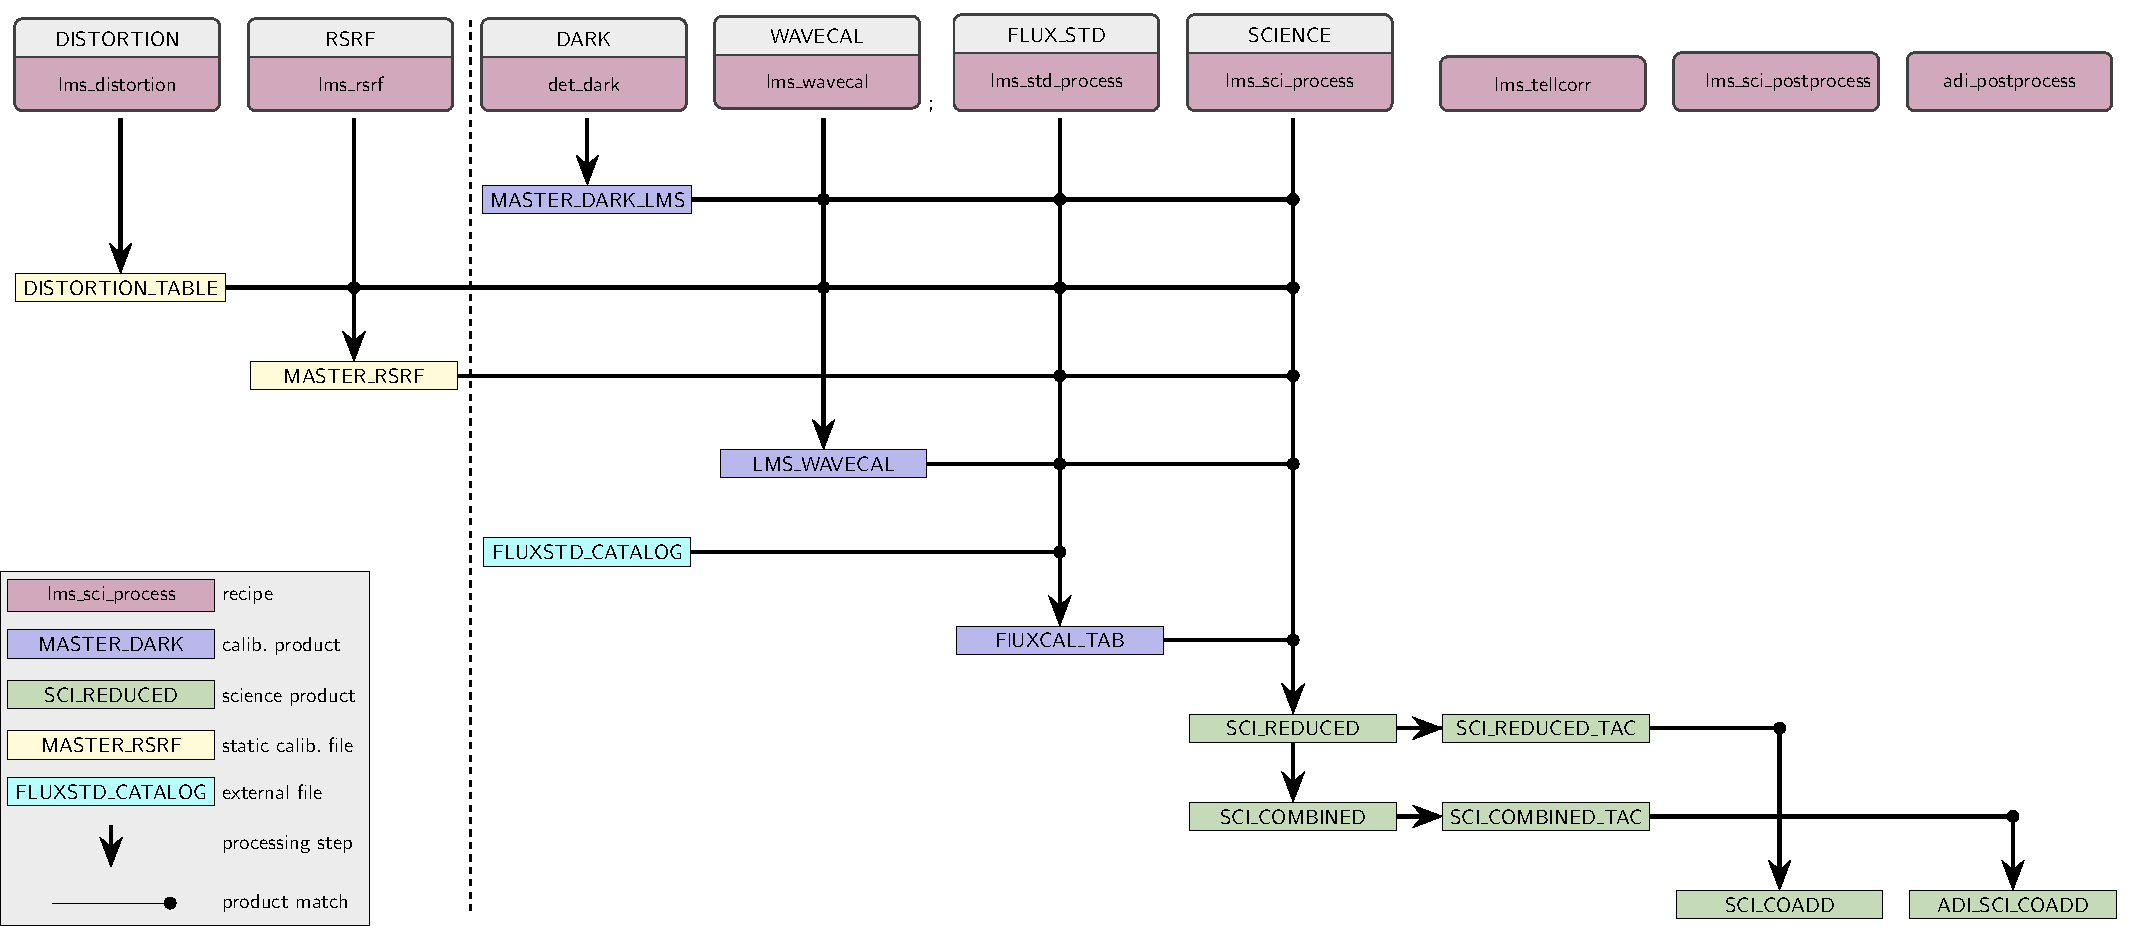
\includegraphics[width=\textheight]{LMS_assomap_tikz}
  \caption[Reduction cascade and association map for IFU
  spectroscopy]{%
    Association map for IFU spectroscopy in L- and M-band (LMS). The
    figure shows only the primary products created by each recipe; for
    a full list of products refer to the recipe descriptions in
    Sect.~\ref{ssec:LMS_recipes}. The dashed lines separates
    calibration tasks that are done at AIT or infrequently during
    operations from daily tasks. The prefix ``\REC{metis_}'' has been
    omitted from the recipe names to improve clarity.}
  \label{Fig:IfuAssomap}
\end{sidewaysfigure}



%%%%%%%%%%%%%%%%%%%%%%%%%%%%%%%%%%%%%%%%%%%%%%%%%%%%%%

%%% Local Variables:
%%% TeX-master: "METIS_DRLD"
%%% End:
